\section{Auswertung}
\label{sec:Auswertung}


Die Graphen werden sowohl mit Matplotlib \cite{matplotlib} als auch NumPy \cite{numpy} erstellt. Die Fehlerrechnung wird mithilfe von Uncertainties \cite{uncertainties} durchgeführt.


\begin{table}
	\centering
	\caption{Messdaten der Stromintensitäten des Interferenzmusters eines Einzelspalts bis zum 1. Nebenmaximum}
	\label{tab:tabEinzel}
	\sisetup{table-format=1.2}
	\begin{tabular}{S[table-format=2.2]S[table-format=1.3]S[table-format=1.3]}
		\toprule
		{$\Delta x/10^{-3}\si{\metre}$} & {$I_.{mess}/10^{-7}\si{\ampere}$} & {$I_.{eff}/10^{-7}\si{\ampere}$} \\
		\midrule
		-13.00 & 0.070 & 0.067 \\
		-12.50 & 0.090 & 0.087 \\
		-12.00 & 0.110 & 0.107 \\
		-11.25 & 0.130 & 0.127 \\
		-10.75 & 0.135 & 0.132 \\
		-10.25 & 0.135 & 0.132 \\
		-9.50 & 0.110 & 0.107 \\
		-9.00 & 0.080 & 0.077 \\
		-8.75 & 0.078 & 0.075 \\
		-8.50 & 0.065 & 0.062 \\
		-8.25 & 0.053 & 0.050 \\
		-8.00 & 0.040 & 0.037 \\
		-7.50 & 0.026 & 0.023 \\
		-7.00 & 0.028 & 0.025 \\
		-6.50 & 0.050 & 0.047 \\
		-6.25 & 0.070 & 0.067 \\
		-6.00 & 0.100 & 0.097 \\
		-5.75 & 0.140 & 0.137 \\
		-5.50 & 0.180 & 0.177 \\
		-5.25 & 0.200 & 0.197 \\
		-5.00 & 0.250 & 0.247 \\
		-4.75 & 0.300 & 0.297 \\
		-4.50 & 0.350 & 0.347 \\
		-4.25 & 0.500 & 0.497 \\
		-4.00 & 0.550 & 0.547 \\
		-3.75 & 0.650 & 0.647 \\
		-3.50 & 0.750 & 0.747 \\
		-3.25 & 0.900 & 0.897 \\
		-3.00 & 1.000 & 0.997 \\
		-2.75 & 1.100 & 1.097 \\
		-2.25 & 1.400 & 1.397 \\
		-1.50 & 1.650 & 1.647 \\
		-0.75 & 1.950 & 1.947 \\
		0.00 & 2.250 & 2.247 \\
		\bottomrule
	\end{tabular}

	\label{tab:1}
\end{table}


\begin{table}
	\centering
	\caption{Messdaten der Stromintensitäten des Interferenzmusters eines Doppelspalts bis zum 2. Nebenmaximum}
	\label{tab:tabDoppel1}
	\sisetup{table-format=1.2}
	\begin{tabular}{S[table-format=2.2]S[table-format=1.4]S[table-format=1.4]}
		\toprule
		{$\Delta x/10^{-3}\si{\metre}$} & {$I_.{mess}/10^{-6}\si{\ampere}$} & {$I_.{eff}/10^{-6}\si{\ampere}$} \\
		\midrule
		-5.00 & 0.1600 & 0.1597 \\
		-4.60 & 0.1250 & 0.1247 \\
		-4.40 & 0.0900 & 0.0897 \\
		-4.20 & 0.0570 & 0.0567 \\
		-4.00 & 0.0320 & 0.0317 \\
		-3.80 & 0.0200 & 0.0197 \\
		-3.60 & 0.0160 & 0.0157 \\
		-3.40 & 0.0195 & 0.0192 \\
		-3.20 & 0.0300 & 0.0297 \\
		-3.00 & 0.0800 & 0.0797 \\
		-2.90 & 0.1100 & 0.1097 \\
		-2.80 & 0.1800 & 0.1797 \\
		-2.60 & 0.3500 & 0.3497 \\
		-2.40 & 0.5800 & 0.5797 \\
		-2.20 & 0.7800 & 0.7797 \\
		-2.00 & 0.9000 & 0.8997 \\
		-1.80 & 0.8900 & 0.8897 \\
		-1.60 & 0.7100 & 0.7097 \\
		-1.40 & 0.4600 & 0.4597 \\
		-1.20 & 0.2500 & 0.2497 \\
		-1.00 & 0.1500 & 0.1497 \\
		-0.80 & 0.2500 & 0.2497 \\
		-0.60 & 0.7500 & 0.7497 \\
		-0.50 & 1.0000 & 0.9997 \\
		-0.25 & 2.0000 & 1.9997 \\
		0.00 & 2.9000 & 2.8997 \\
		\bottomrule
	\end{tabular}

	\label{tab:2}
\end{table}

\begin{table}
	\centering
	\caption{Messdaten der Stromintensitäten des Interferenzmusters eines Doppelspalts bis zum 2. Nebenmaximum}
	\label{tab:tabDoppel2}
	\sisetup{table-format=1.2}
	\begin{tabular}{S[table-format=2.2]S[table-format=1.4]S[table-format=1.4]}
		\toprule
		{$\Delta x/10^{-3}\si{\metre}$} & {$I_.{mess}/10^{-6}\si{\ampere}$} & {$I_.{eff}/10^{-6}\si{\ampere}$} \\
		\midrule
		-2.80 & 0.0500 & 0.0497 \\
		-2.60 & 0.1000 & 0.0997 \\
		-2.40 & 0.3000 & 0.2997 \\
		-2.20 & 0.5500 & 0.5497 \\
		-2.00 & 0.6000 & 0.5997 \\
		-1.80 & 0.4000 & 0.3997 \\
		-1.60 & 0.2000 & 0.1997 \\
		-1.40 & 0.4500 & 0.4497 \\
		-1.20 & 1.2000 & 1.1997 \\
		-1.00 & 1.8000 & 1.7997 \\
		-0.80 & 2.0000 & 1.9997 \\
		-0.60 & 1.3500 & 1.3497 \\
		-0.50 & 0.8000 & 0.7997 \\
		-0.30 & 0.4000 & 0.3997 \\
		-0.20 & 0.5000 & 0.4997 \\
		0.00 & 1.4000 & 1.3997 \\
		0.20 & 2.5000 & 2.4997 \\
		0.40 & 2.8000 & 2.7997 \\
		0.60 & 2.0000 & 1.9997 \\
		0.70 & 1.6000 & 1.5997 \\
		0.90 & 0.5000 & 0.4997 \\
		1.00 & 0.3500 & 0.3497 \\
		1.20 & 0.9000 & 0.8997 \\
		1.30 & 1.4000 & 1.3997 \\
		1.50 & 2.0000 & 1.9997 \\
		1.70 & 1.6000 & 1.5997 \\
		1.90 & 1.1000 & 1.0997 \\
		2.00 & 0.6000 & 0.5997 \\
		2.20 & 0.2000 & 0.1997 \\
		2.40 & 0.2500 & 0.2497 \\
		2.60 & 0.5000 & 0.4997 \\
		2.80 & 0.6000 & 0.5997 \\
		3.00 & 0.4500 & 0.4497 \\
		\bottomrule
	\end{tabular}

	\label{tab:3}
\end{table}

\begin{figure}
\centering
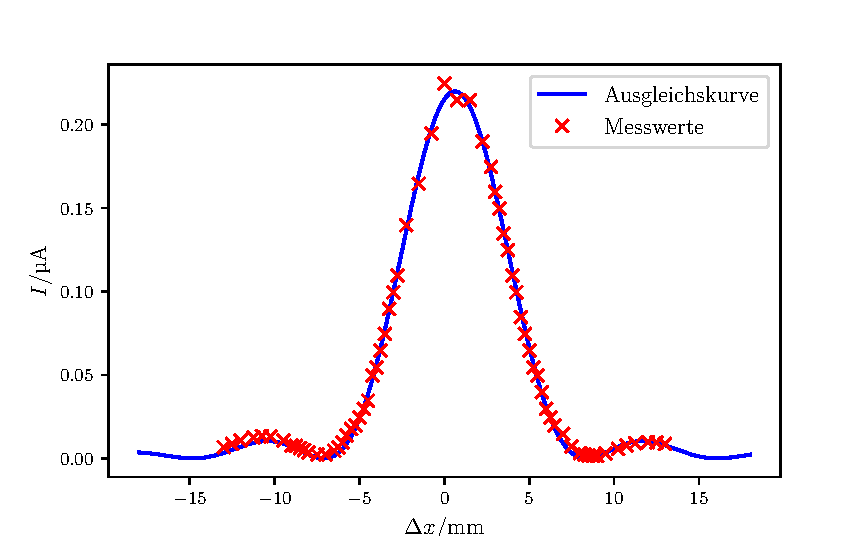
\includegraphics[width=\linewidth-70pt,height=\textheight-70pt,keepaspectratio]{content/images/Einzelspalt.pdf}
\caption{Stromintensitäten des Interferenzmusters eines Einzelspalts in Abhängigkeit von der Verschiebung des Detektors}
\label{fig:Einzel}
\end{figure}

\begin{figure}
\centering
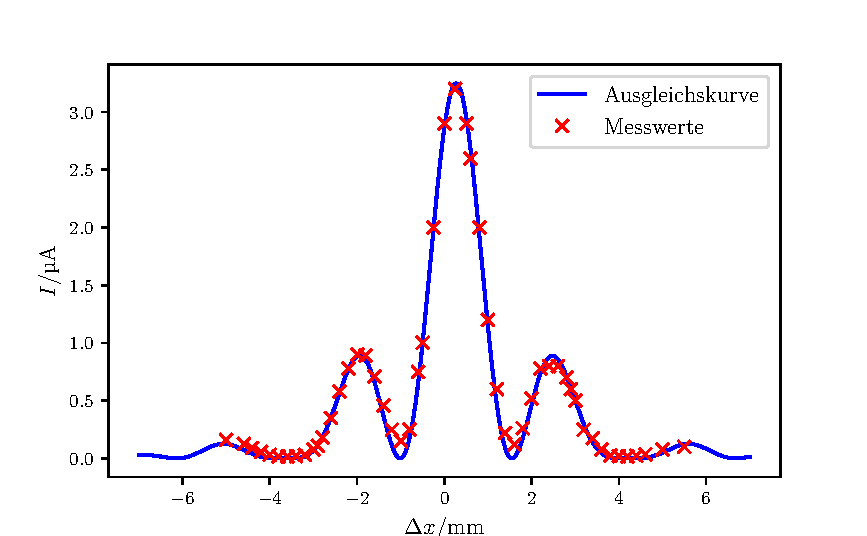
\includegraphics[width=\linewidth-70pt,height=\textheight-70pt,keepaspectratio]{content/images/Doppelspalt1.pdf}
\caption{Stromintensitäten des Interferenzmusters eines Doppelspalts in Abhängigkeit von der Verschiebung des Detektors}
\label{fig:Doppel1}
\end{figure}

\begin{figure}
\centering
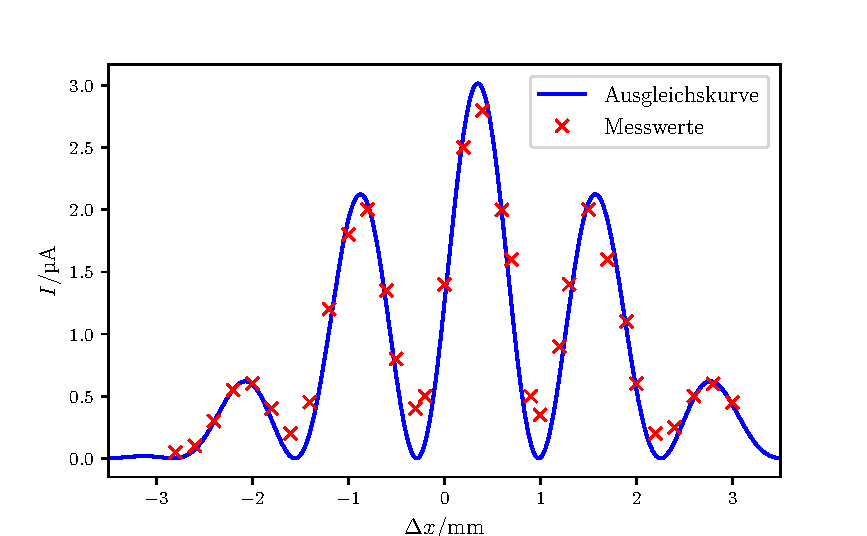
\includegraphics[width=\linewidth-70pt,height=\textheight-70pt,keepaspectratio]{content/images/Doppelspalt2.pdf}
\caption{Stromintensitäten des Interferenzmusters eines Doppelspalts in Abhängigkeit von der Verschiebung des Detektors}
\label{fig:Doppel2}
\end{figure}